\section{Escalamiento en Frecuencia}

\subsection{Análisis del Circuito Prototipo}
En esta fase, se utilizó el mismo circuito base de la parte anterior para estudiar el efecto del desplazamiento en el eje de frecuencias. Se identificó que la tensión en el condensador alcanza su valor máximo a una frecuencia de operación de $158.5 \, kHz$.

\begin{figure}[H]
	\centering
	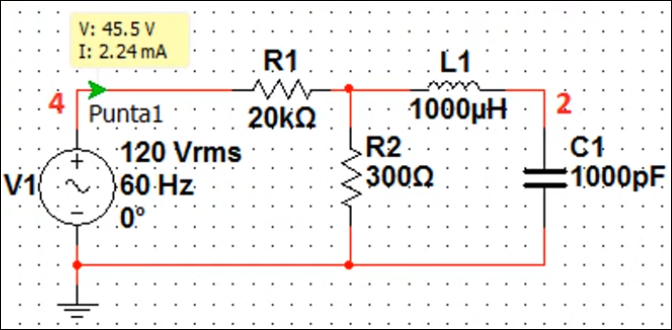
\includegraphics[width=0.7\linewidth]{assets/img/circuito_v2_1.png}
	\caption{Configuración del circuito prototipo para escalamiento en frecuencia.}
	\label{fig:circuito_freq_orig}
\end{figure}

\subsubsection{Resultados de la Simulación Inicial}
Al realizar un análisis de CA a la frecuencia de resonancia identificada ($158.5 \, kHz$), se obtuvieron los siguientes parámetros iniciales:
\begin{itemize}
	\item \textbf{Frecuencia de referencia ($f_{OLD}$):} $158.5 \, kHz$.
	\item \textbf{Impedancia de entrada ($|Z_1|$):} $20 \, k\Omega$ con una fase de $-23.6 \, m^\circ$.
	\item \textbf{Respuesta en frecuencia:} El diagrama de Bode muestra el pico de magnitud exactamente en $158.48 \, kHz$.
\end{itemize}

\begin{figure}[H]
	\centering
	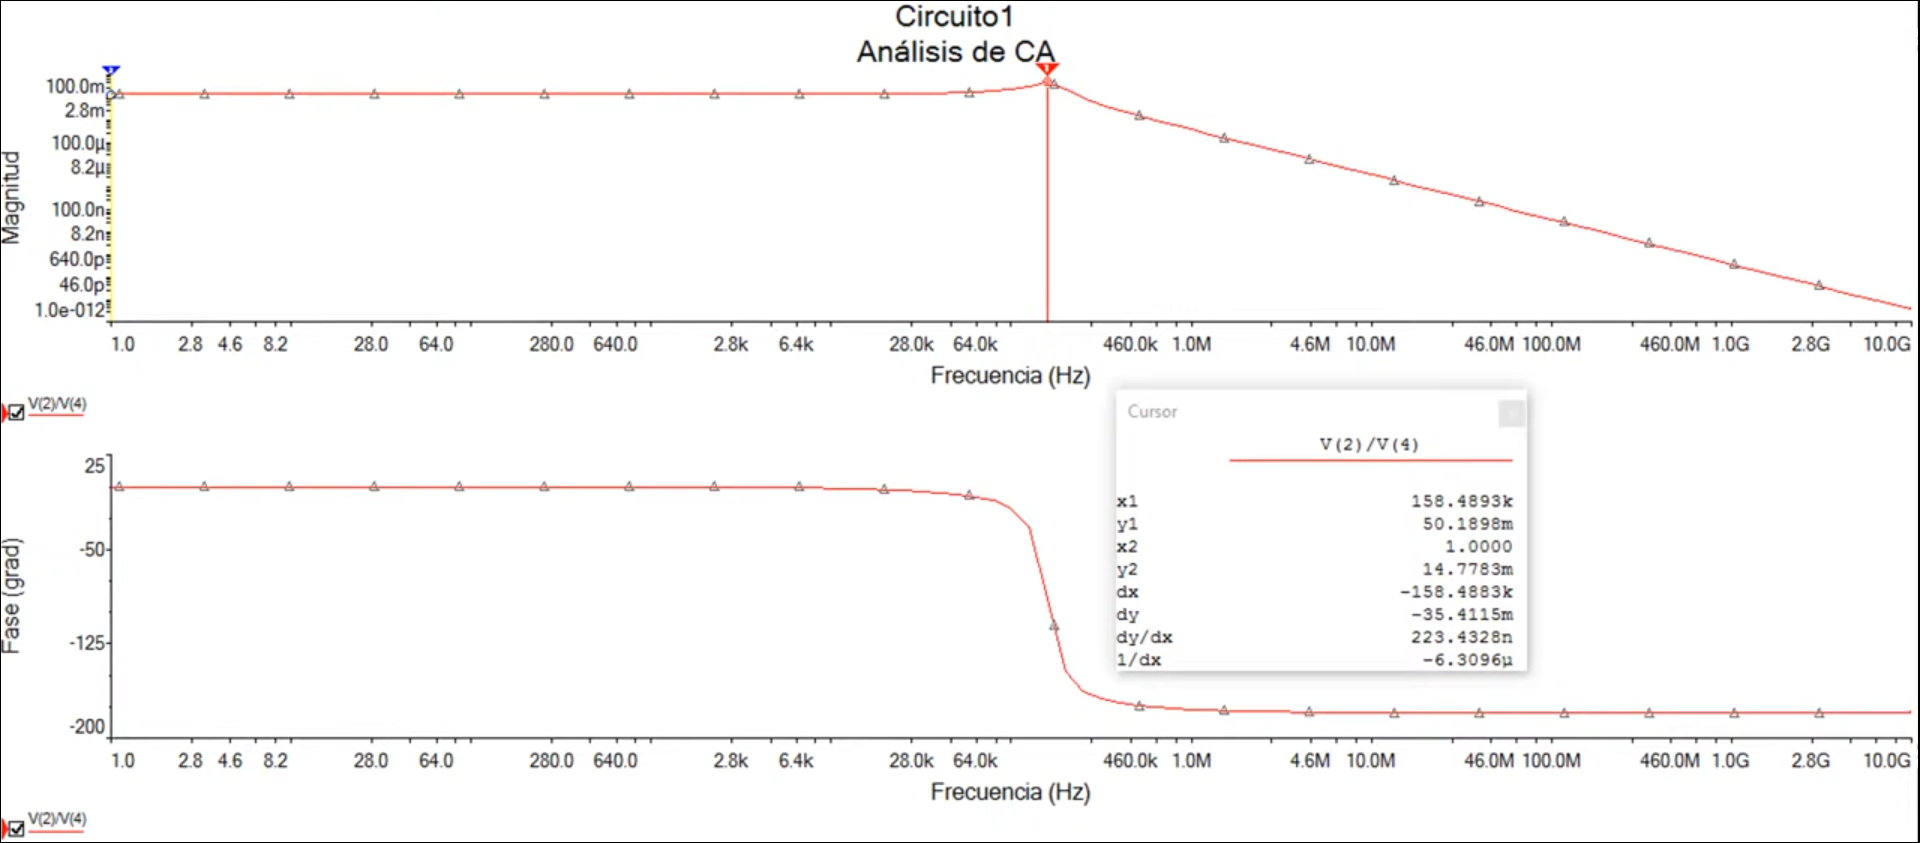
\includegraphics[width=0.7\linewidth]{assets/img/diagrama_bodeogf.png}
	\caption{Diagrama de bode del circuito original.}
	\label{fig:diagrama_bodeogf}
\end{figure}

\subsubsection{Obtención de la Función de Transferencia del Circuito Prototipo}
Para el análisis en el dominio de la frecuencia compleja $s$, se considera el circuito prototipo alimentado por la fuente $V_{in} = V_4$ y se define la salida como el voltaje en el condensador $V_{out} = V_2$. Las impedancias de los elementos se expresan como $Z_R = R$, $Z_L = sL$ y $Z_C = \frac{1}{sC}$.

Aplicando la ley de tensiones de Kirchhoff (LVK) para las mallas del circuito:
\begin{enumerate}
	\item \textbf{Malla 1:} $(R_1 + R_2)I_1 - R_2 I_2 = V_{in}$
	\item \textbf{Malla 2:} $-R_2 I_1 + (R_2 + sL_1 + \frac{1}{sC_1})I_2 = 0$
\end{enumerate}

De la ecuación de la malla 2, despejamos la corriente $I_1$ en función de $I_2$:
\begin{equation}
	I_1 = \frac{s^2 L_1 C_1 + s C_1 R_2 + 1}{s C_1 R_2} I_2
\end{equation}

Sustituyendo $I_1$ en la ecuación de la malla 1 y agrupando términos, se obtiene la expresión para la corriente de la segunda malla $I_2$:
\begin{equation}
	I_2 = \frac{s C_1 R_2 V_{in}}{s^2 L_1 C_1 (R_1 + R_2) + s C_1 R_1 R_2 + (R_1 + R_2)}
\end{equation}

Sabiendo que el voltaje de salida es $V_{out} = I_2 \cdot Z_{C1}$, sustituimos la expresión de $I_2$:
\begin{equation}
	V_{out} = I_2 \cdot \frac{1}{s C_1} = \frac{R_2 V_{in}}{s^2 L_1 C_1 (R_1 + R_2) + s C_1 R_1 R_2 + (R_1 + R_2)}
\end{equation}

Por lo tanto, la función de transferencia $H(s)$ del circuito original es:
\begin{equation}
	H(s) = \frac{V_2}{V_4} = \frac{R_2}{s^2 L_1 C_1 (R_1 + R_2) + s C_1 R_1 R_2 + (R_1 + R_2)}
\end{equation}

\subsection{Aplicación del Escalamiento en Frecuencia ($k_f = 2$)}
El objetivo es desplazar la respuesta del sistema para que actúe de igual manera en una frecuencia diferente. 

Se definió un factor de escalamiento $k_f = 2$, buscando que la nueva frecuencia de operación sea $f' = 317 \, kHz$.De acuerdo con la teoría de escalamiento en frecuencia, la impedancia debe mantenerse igual, por lo que los componentes se modifican según:\begin{equation}R' = R, \quad L' = \frac{L}{k_f}, \quad C' = \frac{C}{k_f}\end{equation}

Calculando los nuevos valores para $k_f = 2$:
\begin{itemize}
	\item $R_1' = 20 \, k\Omega, \quad R_2' = 300 \, \Omega$ (Sin cambios).
	\item $L_1' = \frac{1000 \, \mu H}{2} = 500 \, \mu H$.
	\item $C_1' = \frac{1000 \, pF}{2} = 500 \, pF$.
\end{itemize}

\subsection{Verificación y Comparación de Resultados}
Se implementó el circuito escalado en el simulador para verificar el desplazamiento de la respuesta.

\begin{figure}[H]
	\centering
	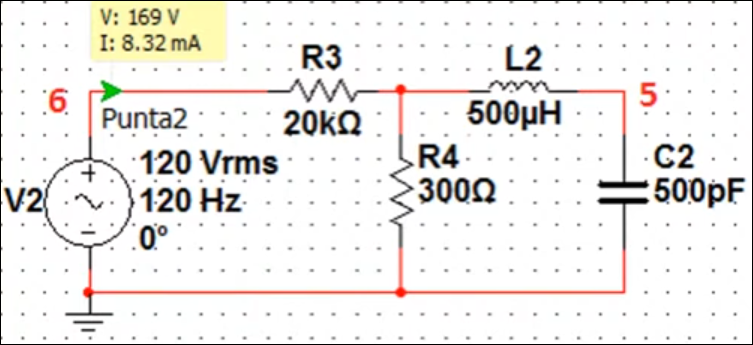
\includegraphics[width=0.7\linewidth]{assets/img/circuito_v2_2.png}
	\caption{Circuito escalado en frecuencia con factor $k_f = 2$.}
	\label{fig:circuito_freq_esc}
\end{figure}

\begin{figure}[H]
	\centering
	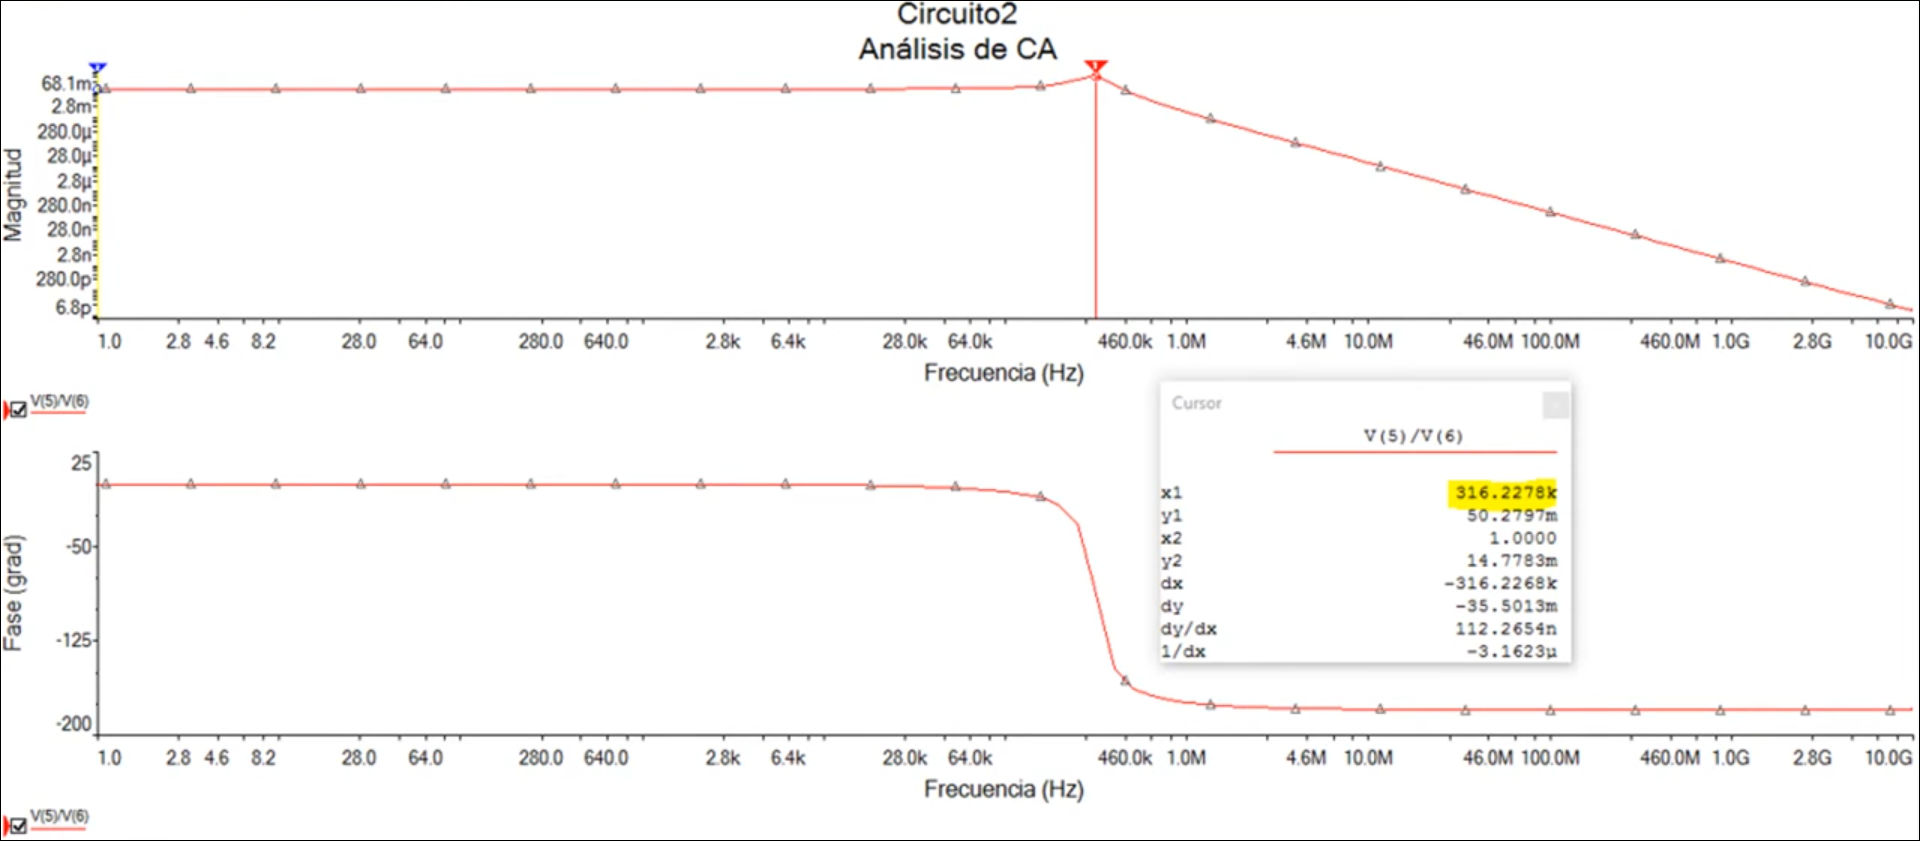
\includegraphics[width=0.7\linewidth]{assets/img/diagrama_bodeescf.png}
	\caption{Diagrama de bode del circuito escalado.}
	\label{fig:diagrama_bodeescf}
\end{figure}

\subsubsection{Análisis de Impedancia y Salida}
Se realizó una medición de la impedancia de entrada a la nueva frecuencia de $317 \, kHz$. Los resultados muestran que $|Z_2| = 20 \, k\Omega$ con una fase de $-23.6 \, m^\circ$. Esto confirma que la impedancia del circuito se mantiene idéntica a la original a pesar del cambio en la frecuencia de operación.

\subsubsection{Validación por Diagramas de Bode}
La comparación de los cursores en los diagramas de Bode confirma el desplazamiento exacto. Mientras que el primer circuito presenta su máximo en $158.5 \, kHz$, el segundo circuito lo presenta en $316.22 \, kHz$ (aproximadamente $317 \, kHz$), lo cual corresponde a la relación $f_{NEW} = k_f \cdot f_{OLD}$.

\begin{figure}[H]
	\centering
	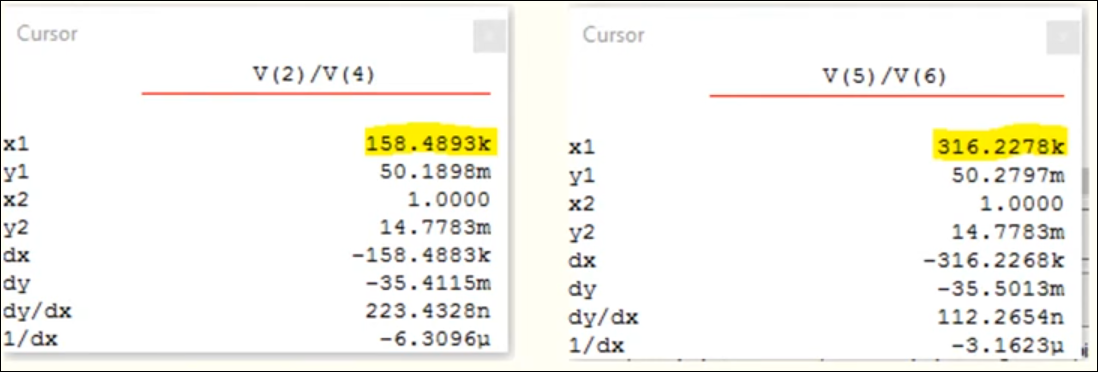
\includegraphics[width=0.7\linewidth]{assets/img/comparacion_cursoresf.png}
	\caption{Comparación de cursores.}
	\label{fig:comparacion_cursores}
\end{figure}

\subsubsection{Análisis Comparativo de la Función de Transferencia}
Para validar analíticamente el efecto del escalamiento en frecuencia, se comparó la respuesta del circuito original $H(s)$ frente a la del circuito escalado $H'(s)$. En este proceso, se aplicó un factor de escala $k_f = 2$, lo que implica que los componentes se transforman de acuerdo con las relaciones $R' = R$, $L' = \frac{L}{k_f}$ y $C' = \frac{C}{k_f}$.

Partiendo de la expresión general de la función de transferencia obtenida mediante el método de mallas para el circuito escalado:
\begin{equation}
	H'(s) = \frac{R_2'}{s^2 L_1' C_1' (R_1' + R_2') + s C_1' R_1' R_2' + (R_1' + R_2')}
\end{equation}

Sustituyendo los valores de los componentes escalados en términos de los originales y el factor $k_f$:
\begin{equation}
	H'(s) = \frac{R_2}{s^2 \left(\frac{L_1}{k_f}\right) \left(\frac{C_1}{k_f}\right) (R_1 + R_2) + s \left(\frac{C_1}{k_f}\right) R_1 R_2 + (R_1 + R_2)}
\end{equation}

Al reorganizar los términos para agrupar el factor $k_f$ con la variable compleja $s$, obtenemos:
\begin{equation}
	H'(s) = \frac{R_2}{\left(\frac{s}{k_f}\right)^2 L_1 C_1 (R_1 + R_2) + \left(\frac{s}{k_f}\right) C_1 R_1 R_2 + (R_1 + R_2)}
\end{equation}

Por inspección, se observa que esta expresión es matemáticamente idéntica a la función de transferencia original, pero evaluada en una frecuencia compleja escalada por el factor $1/k_f$:
\begin{equation}
	H'(s) = H\left(\frac{s}{k_f}\right)
\end{equation}

\textbf{Comparación y Resultados:}
A diferencia del escalamiento de impedancia (donde $H'(s) = H(s)$), el escalamiento en frecuencia produce un desplazamiento directo sobre el eje de las abscisas en el diagrama de Bode. El análisis algebraico anterior demuestra que:
\begin{itemize}
	\item La estructura y la ganancia máxima del circuito no cambian, ya que el factor $k_f$ solo afecta a los términos asociados a la variable $s$.
	\item Al ser $H'(s) = H(s/k_f)$, todas las frecuencias características del sistema (como la frecuencia de resonancia $f_0$ y el ancho de banda) se ven multiplicadas por $k_f$.
	\item Esto explica por qué el pico de tensión en el condensador se desplazó de $158.5 \, kHz$ a exactamente $317 \, kHz$ en la simulación, manteniendo una impedancia constante de $20 \, k\Omega$ en ambos puntos de operación.
\end{itemize}

